\chapter{Algoritmos sustracción del fondo}

\section{Introducción}


La idea en general del proceso de sustracción de fondo es modelar cada uno de los píxeles de una escena mediante una función de densidad de probabilidad. Esto se apoya en la suposición que las imágenes de una escena sin objetos en circulación, tiene un comportamiento regular que puede ser descrito por un modelo estadístico. Un evento podría ser detectado identificando las partes de la imagen que no se ajustan con el modelo que describe el fondo. El píxel de una nueva imagen sólo se considera parte del fondo, si el valor queda completamente descrito por la función de densidad de probabilidad. 

Esta sección hace una presentación de los algoritmos que emplean modelos estadísticos para describir el segundo plano de una secuencia. Se detalla el modelo de Mixtura de Gaussianas propuesto por \textit{Zivkovic y Heidjen} \cite{zivkovic_efficient_2006}, y la mejora propuesta por \textit{Zezhi Chen} \cite{chen_vehicle_2012}. Se describe además el modelo no-parametrico de \textit{Elgammal} \cite{elgammal_nonparametricmodel_2000}.


\section{Modelo General}

La intensidad de un píxel en el tiempo (o en el transcurso de una secuencia) es utilizada para construir una función de densidad de probabilidad, que corresponde al modelo descriptivo de la distribución de ese píxel en específico. El modelo es una combinación lineal de un conjunto de distribuciones Gaussianas. Cada componente Gaussiano del modelo es caracterizado por un grupo de parámetros que identifica los elementos que aparecen en el avance de las imágenes.

\begin{figure}[h!]
  \centering
      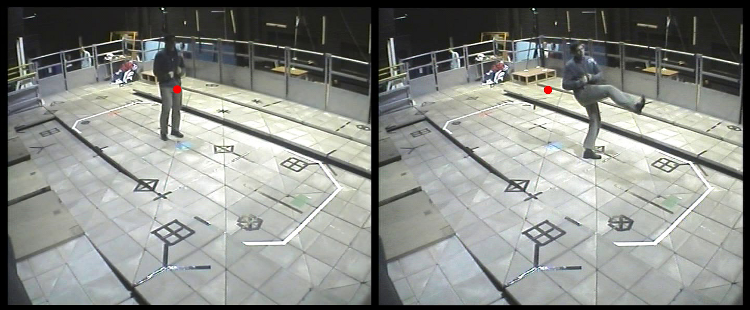
\includegraphics[scale=0.5]{img/figura_3_1}
  \caption[Imágenes 120, 180 de secuencia ``\textit{Kick Camera 3 Person 4}'']{Imágenes 120 y 180 de la secuencia MuHAVI-MAS ``\textit{Kick Camera 3 Person 4}''. El punto en rojo señala la misma posición de un píxel en dos eventos diferentes}
\label{posicion_340_160}
\end{figure}

Para comprender el principio de clasificación de píxeles entre elementos del fondo y otros objetos, La figura ~\ref{posicion_340_160} muestra dos imágenes de la secuencia MuHAVI-MAS \textit{``Kick Camera 3 Person 4''}\cite{singh_muhavi_2010}. Ambos cuadros señalan el estado de un píxel (punto rojo) en dos instantes diferentes. La primera imagen el punto forma parte del escenario (\textit{background}), y el valor de intensidad del píxel, queda determinado por los colores del escenario. La siguiente imágen el punto es parte del actor en movimiento (\textit{foreground}), por lo que el valor del píxel será el de los colores de la ropa del actor. La figura ~\ref{intensidad_340_160} muestra la intensidad del color rojo en la secuencia completa, 730 imágenes, del píxel. Se debe recordar que el valor de un píxel se define como un vector de tres componentes en el espacio de colores RGB, en la figura ~\ref{intensidad_340_160} sólo se muestra el valor de color rojo.

\begin{figure}[h!]
  \centering
      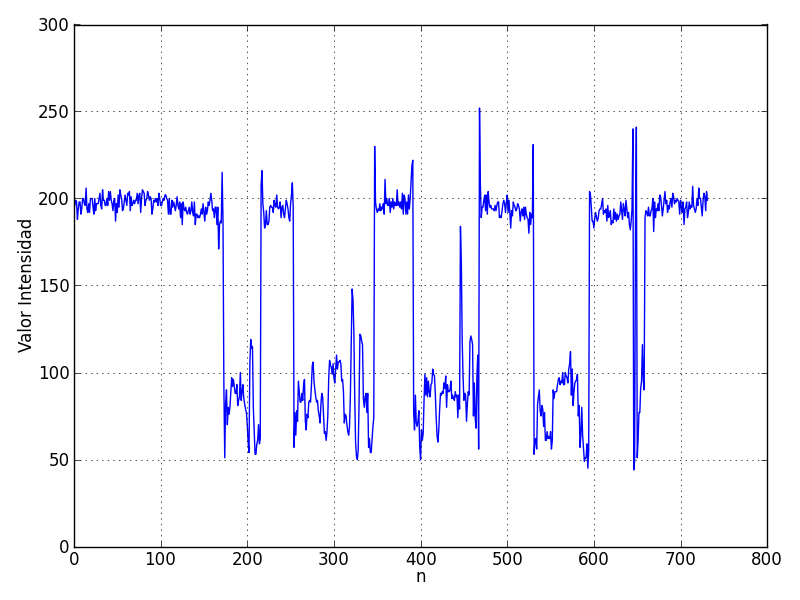
\includegraphics[scale=0.5]{img/figura_3_2}
  \caption[Intensidad en el tiempo de un pixel ]{Intensidad del píxel rojo en el tiempo de la secuencia completa.}
\label{intensidad_340_160}
\end{figure}



La gráfica de la figura ~\ref{intensidad_340_160} señala el comportamiento del píxel en la secuencia completa. Se puede apreciar por ejemplo, que el actor cruza en varias oportunidades la ubicación del píxel, los valores entre el rango de 50 y 100 es un indicio de esto, debido principalmente que los colores de la ropa del actor son más oscuros y son valores más espaciado. El escenario presenta al contrario, rango de valores más constantes con menor varianza que los colores del actor. Estas características permiten construir un modelo basado en mixtura de Gaussianas para clasificar elementos de la imágen. Los parámetros que describen cada uno de las componentes Gaussianos son los factores que posteriormente se utilizan para realizar clasificación. 

\begin{figure}[h!]
  \centering
      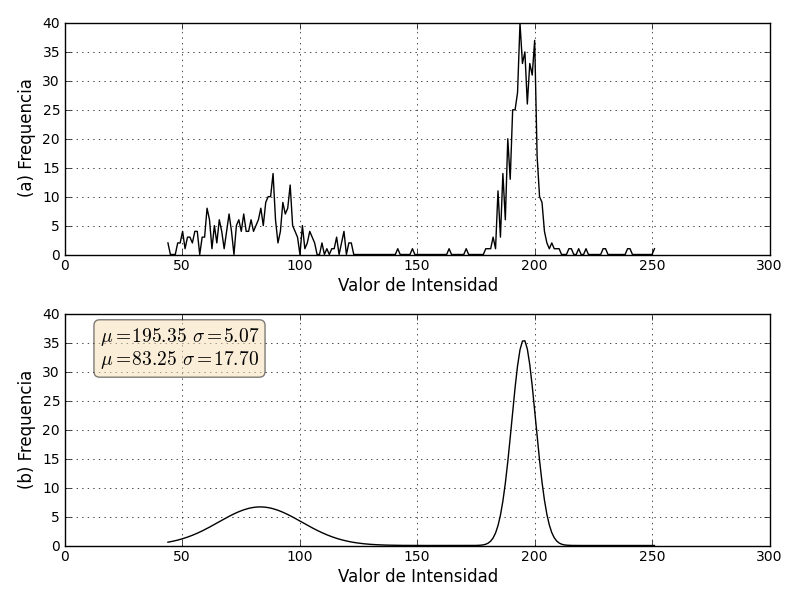
\includegraphics[scale=0.75]{img/histograma_pixel_340_160_3_2}
  \caption[Histograma píxel rojo]{Histograma píxel rojo de la secuencia completa}
\label{histograma}
\end{figure}


El modelo de la secuencia completa de este pixel se describe por el histograma de la figura ~\ref{histograma} (a). En esta imagen se pueden distinguir dos formas bien definidas: un tipo se asocia con el fondo de imagen y el otro con el actor en movimiento. La mixtura de Gaussianas se construye, para este ejemplo, ajustando la función de densidad a dos distribuciones Gaussianas, figura ~\ref{histograma} (b). De ambas imágenes se pueden señalar un par de cosas que son el fundamento sobre la cual se construyen modelos de mixtura de Gaussianas para sustracción de fondo. En primera instancia el modelo que describe este píxel en particular, queda completamente definido por una función de distribución compuesta de dos Gaussianas. En términos cualitativos se observa que una componente Gaussiana tiene una varianza más reducida (estrecha) con respecto a la otra componente, esta característica permite asociar este componente con la imagen de fondo. Otro aspecto importante es la frecuencia de ambos componentes, el menor valor de frecuencia se asocia con el actor en movimiento, esto debido que el actor es un elemento dinámico y pasa menos tiempo en el escenario. El escenario es constante no se mueve, por lo que se debiera reflejar en la frecuencia de mayor valor.

Tomando en cuenta estos factores, el algoritmo de sustracción de fondo puede discriminar el píxel del fondo de imagen y un objeto que se está moviendo. Cualquier pixel con una componente Gaussiana que no se ajuste a la distribución de menor varianza se considera objeto en movimiento. Sin embargo, si este mismo objeto queda estático por un tiempo considerable, su distribución Gaussiana comenzará a mostrar un varianza similar a la varianza del fondo, en ese momento el píxel se considera parte del fondo.






\section{Mixtura de distribuciones Gaussianas - GMM}


La superposición de distribuciones Gaussianas que describen el comportamiento de un pixel, se define en la ecuación \eqref{eq:mixturegaussians}. Esta es una sumatoria de \textit{``K''} componentes Gaussianos $\mathcal{N}( x | \mu_k , \Sigma_k)$, cada uno ponderado por un factor multiplicativo $\pi_k$, la cual establece una función de densidad de probabilidad general para el píxel $p(x)$. El factor de ponderación $\pi_k$ es el grado de influencia de cada componente, en el comportamiento global del píxel que esta siendo modelado. Los valores de ponderación pueden ser interpretados, como probabilidades de ocurrencias de las diferentes clases, Background y Foreground, representadas por los diferentes componentes Gaussianos; por ejemplo, $\pi_1$ podría representar la probabilidad que un píxel sea la imagen de fondo. La suma total de los factores $\pi_k$ es 1, indicado en la ecuación \eqref{eq:mixturefactor}. 

\begin{equation} \label{eq:mixturegaussians}
p(x) = \sum_{k=1}^{K} \pi_k \mathcal{N}( x | \mu_k , \Sigma_k)
\end{equation}

\begin{equation} \label{eq:mixturefactor}
\sum_{k=1}^{K} \pi_k = 1
\end{equation}


Una de las principales tareas del algoritmo que implementa mixtura de Gaussianas, es mantener actualizado los $K$ valores estimados de media ($\mu_1, ..., \mu_k$),  covarianza ($\Sigma_1, ..., \Sigma_k$) y el factor de ponderación ($\pi_1, ..., \pi_k$), por cada píxel de una nueva imagen. Se utilizan los valores de intensidad en el espacio de colores RGB, para construir la mixtura de componentes Gaussianas de un píxel.

La estimación de los parámetros $\vec{\theta} = \{\pi_1,..,\pi_k, \mu_1,..,\mu_k,\Sigma_1,..,\Sigma_k \} $ de las distintas mixturas se realiza mediante el método de Máxima Verosimilitud (\textit{Maximum Likelihood Estimate - MLE}). De esta manera, los parámetros estimados por máxima verosimilitud de un conjunto $t$ de muestras $\mathcal{X} = \{\vec{x}^{(1)}, ..., \vec{x}^{(t)}\}$, quedan determinados por la ecuación (~\ref{eq:maxima_verosimilutd}). Una explicación bien detallada de estimación mediante el método de máxima verosimilitud se puede ver en el capítulo 3 de la referencia \cite{duda_pattern_2000}.

\begin{equation} \label{eq:maxima_verosimilutd}
\hat{\vec{\theta}} = arg \max_{\vec{\theta}}  (\log p(\mathcal{X};\vec{\theta}))
\end{equation}

 
Debido a la dificultad de encontrar una solución analítica de \textit{MLE}, se emplea una aproximación numérica iterativa para maximizar la función de verosimilitud.  El algoritmo de esperanza-maximización (EM) \cite{dempster_maximum_1977} se usa para encontrar soluciones de máxima verosimilitudes. Este es un procedimiento iterativo que busca un máximo local de la función log-verosimilitud. Este algoritmo es fácil de implementar, sin embargo una de sus limitaciones es la posibilidad de converger en un pobre máximo local que no fue apropiadamente inicializado.


\subsection{Actualización parametros del Algoritmo}

Esta sección describe el procedimiento empleado en el trabajo de \textit{Zivkovic y Heidjen} \cite{zivkovic_efficient_2006}, que actualiza en forma recursiva las ecuaciones que estiman los párametros $\mu_k$, $\Sigma_k$, $\pi_k$ del componente Gaussiano $K$. Por razones computacionales las matrices de la covarianza son Isotrópicas, matriz de identidad.

Esta aproximación plantea estimar el modelo del fondo desde un conjunto de entrenamiento $X$, el cual mantiene una historia específica de muestras por cada píxel. Para adecuarse a los posibles cambios que puedan producirse en el fondo, el conjunto de entrenamiento es actualizado con nuevas muestras que llegan y simultáneamente descarta las más antigua. Se elige un adecuado periodo de adaptación $T$ (100 cuadros) para mantener una historia reciente del fondo, y en el instante ``$t$'' se tiene el conjunto de entrenamiento $\mathcal{X_T} = \{x^{(t)}, ..., x^{(t-T)}\}$, desde el cual se estima la función de densidad del fondo.

La parte central del algoritmo, consiste en actualizar constantemente los parámetros $\vec{\theta}$ de las distribuciones Gaussianas, que describen el estado de cada píxel en un momento determinado. Las ecuaciones recursivas para estimar los parámetros de una muestra nueva $x^{(t)}$ en tiempo $t$ se presentan a continuación:


\begin{equation} \label{eq:mixturefactor_update}
\hat{\pi}_k \leftarrow  \hat{\pi}_k + \alpha(o^{(t)}_k - \hat{\pi}_k) - \alpha C_T
\end{equation}
\begin{equation} \label{eq:mixturemu_update}
\hat{\vec{\mu}}_k \leftarrow \hat{\vec{\mu}}_k + o^{(t)}_k (\alpha/\hat{\pi}_k) \vec{\delta}_k
\end{equation}
\begin{equation} \label{eq:mixturesigma_update}
\hat{\sigma}^2_k \leftarrow \hat{\sigma}^2_k + o^{(t)}_k (\alpha/\hat{\pi}_k) (\vec{\delta}^T_k \vec{\delta}_k - \hat{\sigma}^2_k)
\end{equation}

\[
\vec{\delta}_k = \vec{x}^{(t)} - \hat{\vec{\mu}}_k
\]


El factor constante $\alpha$ define una curva de decaimiento exponencial para limitar la influencia de la data más antigua. Se usa esta constante como reemplazo de $T$ mencionado anteriormente, relacionando ambas constante por la siguiente relación: $\alpha=1/T$. 

Una nueva muestra se compara con todos los componentes, en caso de 
Se define que una muestra nueva pertenece a algunos de los componentes Gaussianos si el factor $\pi_k$ tiene una distancia de Mahalanobis menor que 3, en este caso el valor de \textit{ownership} se coloca en 1, en caso contrario es 0. Cada nueva muestra que se recibe 


\textcolor{red}{No considerar de esta parte en adelante, todavía falta mejorar}

